\subsection{Systems, from toy to large}

We order the systems by how much control they give us (Table~\ref{tab:systems}). Toy networks trained from scratch let us keep parts new to the system itself and score its own outputs on them, so they test the hypotheses cleanly. Pretrained models saw their parts in pretraining, so parts are new only to the probe. For them we add random weights, training checkpoints and invented words as controls, and we ask whether the toy pattern recurs.

\begin{table}[t]
  \centering
  \small
  \caption{\textbf{Every system supplies parts, wholes and a state, and each supplies an output of its own.} Parts new to the system never entered its training, whereas parts new to the probe entered pretraining while staying out of the probe's fit. Invented words extend the language models' test to parts new to the model itself.}
  \label{tab:systems}
  \begin{tabular}{@{}p{0.14\linewidth}p{0.15\linewidth}p{0.16\linewidth}p{0.16\linewidth}p{0.16\linewidth}p{0.08\linewidth}@{}}
    \toprule
    System & Parts & Whole & State & Own output & New to \\
    \midrule
    Toy operators & Gaussian vectors in $\R^{16}$ & the operator's output on two parts & the output itself & lookup among training parts & probe \\
    Glyph networks & $8 \times 8$ glyphs & two glyphs on a canvas & encoder output $h \in \R^m$ & decoder's rendering & system \\
    Recursive composers & Gaussian leaves in $\R^8$ & binary tree of depth $n$ & root state & recursive decomposer & system \\
    Image encoders & Tiny-ImageNet photographs & two photographs on a canvas & patch states of each quadrant, or their average & matching captions through the pooled embedding, for image--text models & probe \\
    Diffusion models & the same photographs; nouns & a canvas; a caption naming two objects & denoiser features & generated images; choosing captions by denoising error & probe \\
    Language models & 305 concrete nouns & ``a $x$ on a $y$'' & question state; average over tokens & answering role questions & probe \\
    \bottomrule
  \end{tabular}
\end{table}

\paragraph{Glyph networks.} A fixed random generator renders a latent $z \in \R^{8}$ as an $8 \times 8$ glyph, and a whole places two glyphs on an $8 \times 16$ canvas under one of three relations. \textsc{beside} uses disjoint regions, \textsc{over} draws both glyphs in one region with the second mirrored, and \textsc{occlude} draws the second at half scale over the first. An encoder writes a state $h \in \R^m$, and a decoder renders the same parts in the same roles. The state serves as the system's representation, and the decoder as its own output. We train an MLP, a CNN, a transformer and a role--filler network, whose decoder renders each half of $h$ with one shared glyph decoder, at widths $m$ from 8 to 64 and vocabularies $V$ from 8 to 64 glyphs, with 9 seeds. With $V = 8$, two glyphs never fill role~2 in training, which removes 14 of the 56 ordered pairs of distinct glyphs, and a network trains on 34 of the remaining 42 until its training loss nears zero. The other eight pairs of the same glyphs test weak compositionality, and 256 wholes of glyphs outside its training test strong compositionality.

\paragraph{Recursive composers.} Balanced binary trees of depth $n$ carry Gaussian leaves in $\R^8$. A recursive auto-associative memory \citep{pollack1990} applies one learned composer at every node and one learned decomposer recursively, both trained on depths 1 and 2. The decomposer is the system's own output, and a probe maps the same root state to all $2^n$ leaves. For comparison, holographic reduced representations (HRR) of the same width $w$ use one pair of unitary role vectors per level, with 5 seeds for each $w$ from 16 to 256.

\paragraph{Pretrained models.} Sentences place two nouns in the roles of five asymmetric relations, such as ``a $x$ on a $y$'', and of the control ``a $x$ and a $y$''. We split 305 concrete nouns into 165 for training probes, 40 for validation and 100 new to the probe. Photographs come from Tiny-ImageNet \citep{le2015tiny}, whose 200 classes we split into 120, 30 and 50 in the same way. Two photographs share a $224 \times 224$ canvas, \textsc{beside} or \textsc{above} each other, or \textsc{overlap}ping. We test eleven text encoders from CLIP \citep{radford2021clip}, including those that condition Stable Diffusion \citep{rombach2022}, T5 \citep{raffel2020t5}, BERT \citep{devlin2019bert} and GPT-2 \citep{radford2019gpt2}. The image encoders are CLIP ViT-B/32 and ViT-H/14 \citep{radford2021clip,cherti2023}, DINOv2 small, large and giant \citep{oquab2024dinov2}, and SigLIP so400m \citep{zhai2023siglip}. The diffusion models are Stable Diffusion 1.5 and SDXL \citep{rombach2022}. The language models are Qwen3-8B \citep{yang2025qwen3}, OLMo-2 7B and 13B \citep{olmo2024olmo2}, phi-4 \citep{abdin2024phi4}, and seven Pythia models from 160 million to 12 billion parameters \citep{biderman2023pythia}, and the GPT-2 models also answer as language models. We also follow ten checkpoints of Pythia-1.4b, plus nine checkpoints each of Pythia-410m and of five PolyPythia reruns \citep{vanderwal2025polypythias}.

\paragraph{Roles by meaning.} Each relation has a \emph{converse} paraphrase that reverses the order of mention while keeping the meaning, such as ``a tulip on a barrel'' and ``a barrel under a tulip'' (Figure~\ref{fig:protocol}c). The tulip is the \emph{figure} in both sentences, and the barrel is the \emph{ground}. The language models answer questions such as ``Which object is on top?'' after four demonstrations with training nouns. A test prompt ends with ``Sentence: a tulip on a barrel. Question: Which object is on top? Answer: the'', and we call the model's state at that final token the \emph{question state}. Image--text encoders match a canvas against a caption that names its objects in their places and against the same caption with the places swapped. Text encoders match a sentence against its converse paraphrase and against the same paraphrase with the nouns exchanged.

\subsection{Protocol}

\begin{figure}[t]
  \centering
  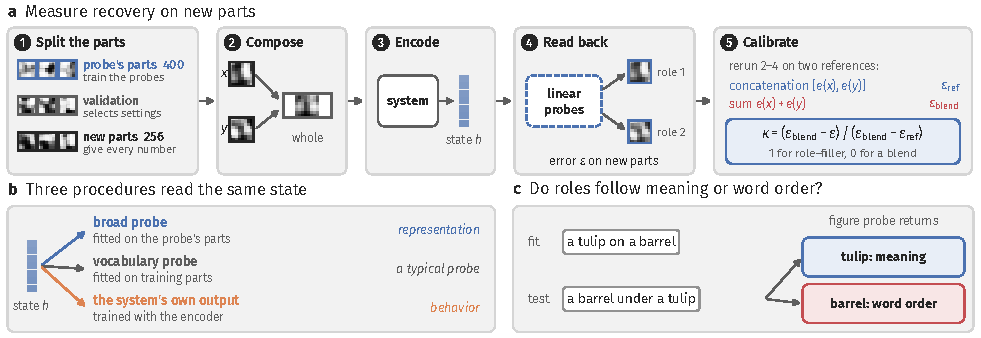
\includegraphics[width=\linewidth]{fig_protocol.pdf}
  \caption{\textbf{One protocol reads the same new parts through three procedures.} \textbf{a.} We split the parts before fitting anything (1). The system encodes wholes of two parts (2, 3), and linear probes fitted on the probe's training parts return each role's part from the state, with error $\varepsilon$ on new parts (4). The same steps, run on the concatenation and on the sum of the same part vectors, calibrate $\varepsilon$ into recoverability $\kappa$ (5). \textbf{b.} A probe trained on many parts measures the representation, a probe trained on the system's training parts stands in for a typical probe, and the system's own output measures behavior. \textbf{c.} A converse paraphrase keeps the figure and reverses the order of mention. A probe of the figure fitted on one phrasing therefore returns the tulip on the other if roles follow meaning, and the barrel if they follow word order. Colors keep one meaning in every figure. Orange marks the system's own output and blue a probe of its state. Green marks a procedure that reads through the state, such as a new decoder, an edit or a patch, grey marks controls and references, and red marks a blend or an answer by word order. Filled markers denote new parts and open markers training parts.}
  \label{fig:protocol}
\end{figure}

We split the parts before we fit anything. Probes and role maps fit wholes built from the probe's training parts, and new parts give every reported number. The probe class is linear and fixed before any result, and validation parts select only the ridge penalty, the layer and the part vector within that class. For a pretrained model, a part vector is the model's state for one part alone (``a $x$'', ``there is a $x$ here'', or the photograph), reduced to 16 principal components, each scaled to unit variance \citep{timkey2021}. For glyph networks, the part vector is the top 16 principal components of the glyph's pixels. Each system also runs with random weights, which keep its architecture, tokenizer and input format but remove learning. Every number is a mean over seeds, and Appendix~\ref{app:protocol} gives further details.

Two probes recur. The \emph{broad probe} trains on many parts, more than the dimension of the part vector, and measures the representation. The \emph{vocabulary probe} trains on the system's own training parts, as a typical probe would, and shows the ceiling that a procedure learned from that vocabulary faces (Proposition~\ref{prop:span}).

\subsection{Metrics}
\label{app:metrics}

Every metric scores wholes built from new parts.
\begin{itemize}
  \item \textbf{Recovery $R^2$.} For a procedure $u$ that returns a part vector, $R^2 = 1 - \varepsilon$ with $\varepsilon$ as in Eq.~\eqref{eq:recover}. The same score applies to probes, decoders and decomposers.
  \item \textbf{Recoverability $\kappa$.} Eq.~\eqref{eq:kappa} rescales a probe's error so that the sum of the part vectors scores 0 and their concatenation scores 1.
  \item \textbf{Role transfer.} A probe of the figure fits canonical sentences and reads converse ones. Role transfer is the share of converse sentences whose prediction $\hat{e}$ lies nearer the figure's vector than the ground's. Roles by meaning score 1, and word order scores 0.
  \item \textbf{Answer accuracy.} The share of questions on which the model prefers the correct noun by summed log-probability. Half of the questions ask for the figure and half for the ground, in both phrasings, so answering by word order scores 0.5.
  \item \textbf{Flip rate.} The share of pairs whose answer changes to the source's answer when we patch the question state, or one subspace of it, from a source prompt with the opposite figure.
  \item \textbf{Role residual $\delta$.} The share of a state's variance that the role maps of Eq.~\eqref{eq:factor} leave unexplained, so one shared code per role scores 0.
\end{itemize}
